\section{Результаты апробации решения}

%TODO: описать, откуда взяты данные

\subsection{Конфигурация тестовой ЭВМ}
\label{subsec:test_stand}

\begin{itemize}
 \item Процессор: Intel Core i5-3320M, 2.6 ГГц;
 \item ОЗУ: 1024 МБ;
 \item ОС: Debian Linux 7 (wheezy), 32-разрядная.
\end{itemize}

Тестирование решения проводилось на виртуальной ЭВМ в среде Oracle VM 
VirtualBox [\ref{virtualbox}].


\subsection{Генератор трасс}

Для проверки общей работоспособности решения без доступа к реальным 
или смоделированным ВС полезно провести апробацию средства на данных, 
полученных с помощью генератора трасс обменов.

Такой генератор был разработан ранее для демонстрационных целей. Для 
передачи данных агенту Анализатора МКИО используется специальное виртуальное 
устройство-петля. С помощью генератора можно получить последовательности 
обменов, подходящие для проверки возможностей анализатора ограничений.

Во время работы генератор непрерывно передаёт набор сообщений определённых 
типов и содержания с  частотой. 

Перечень генерируемых параметров приведён в таблице~\ref{tab:params}. Для 
каждого параметра приводится функция значения, а также описание 
обмена, передающего значение параметра (адреса и подадреса отправителя и 
получателя, формат сообщения, размер сообщения, номер первого слова, номер 
первого бита и длина битового поля). Параметры по умолчанию целочисленные.

Значение $i$ в определении функции - значение целочисленного счётчика, 
увеличиваемое на 1 каждый промежуток времени, заданный в исходном коде 
генератоа (по умолчанию - 300 мс).

Легенда таблицы:

\begin{itemize}
 \item $A_{src}$ - адрес источника сообщения (0-31, либо КК - контроллер 
канала);
 \item $SA_{src}$ - подадрес источника сообщения (0-30, либо КК - контроллер 
канала);
 \item $A_{dst}$ - адрес получателя сообщения (0-31, либо КК - контроллер 
канала);
 \item $SA_{dst}$ - подадрес получателя сообщения (0-30, либо КК - контроллер 
канала);
 \item $Sz_{msg}$ - размер сообщения (количество слов);
 \item $St_{word}$ - номер слова, в котором начинается битовое поле параметра;
 \item $St_{bit}$ - номер первого бита битового поля параметра в этом слове;
 \item $Sz_{bf}$ - количество бит в битовом поле параметра;
 \item $Sc$ - цена младшего бита битового поля.
\end{itemize}

\begin{table}[H]
\centering
\begin{tabular}{|l|l|*{9}{c|}}
\hline
 № & Функция & $A_{src}$ & $SA_{src}$ & $A_{dst}$ & $SA_{dst}$ & $Sz_{msg}$ & 
$St_{word}$ & $St_{bit}$ & $Sz_{bf}$ & $Sc$ \\
\hline
1 & $10^6 * sin(i / 10)$ & КК & КК & 2 & 1 & 4 & 0 & 0 & 32 & 1.0 \\
2 & $i$; 0x42 & КК & КК & 2 & 1 & 4 & 2 & 0 & 16 & 1.0 \\
3 & $10^6 * sin(i / 10)$ & КК & КК & 2 & 3 & 4 & 0 & 0 & 32 & 1.0 \\
4 & $i$; 0x42 & КК & КК & 2 & 3 & 4 & 2 & 0 & 16 & 1.0 \\
5 & $10^6 * sin(i / 10)$ & КК & КК & 2 & 4 & 4 & 0 & 0 & 32 & 1.0 \\
6 & $i$; 0x42 & КК & КК & 2 & 4 & 4 & 2 & 0 & 16 & 1.0 \\
\hline 
\end{tabular}
\caption{Перечень параметров, предоставляемых генератором}
\label{tab:params}
\end{table}

В значения некоторых параметров генератором вносятся ошибки. Ошибки 
для таких параметров описаны в таблице~\ref{tab:param_errors}. Частота 
возникновения здесь - количество циклов генератора, определяемых частотой 
увеличения внутреннего целочисленного счётчика $i$. $rnd()$ - значение, 
определяемое с помощью генератора псевдослучайных чисел (функции 
\textit{random()} стандартной библиотеки языка Си).

\begin{table}[H]
 \centering
 \begin{tabular}{|l|c|c|}
  \hline
  № & Ошибочное значение & Частота возникновения \\
  \hline
  5 & побитовое НЕ верного значения & $rnd()$ \\
  6 & 0xDEAD & 10 \\
  \hline
 \end{tabular}
 \caption{Ошибочные значения параметров}
 \label{tab:param_errors}
\end{table}

\subsection{Примеры описаний протоколов и апробация}

Апробация возможностей анализатора ограничений проводилась на наборе примеров 
описаний протоколов и ограничений, соответствующих трассам обменов, полученным 
с помощью генератора.

Ниже приводятся примеры описаний протоколов, графики значений параметров, 
описанных в этих протоколах и результаты работы анализатора для этих 
описаний протоколов. Проверка работы анализатора проводилась в режиме 
регистрации обменов в реальном времени.

\subsubsection{Пример 1}

В примере 1 наблюдается изменение значений младших 8 бит значений параметров 4 
и 6 из таблицы~\ref{tab:params} (назовём полученные параметры 4а и 6а 
соответственно). Значение параметра 4а 
постоянно и равно 42. Если для параметра 6а не выполнено условие генерации 
ошибки, его значение равно значению параметра 4а, иначе - константе 173 (0xAD). 

Параметры связываются в группу с идентификатором \textit{int42} со 
значениями погрешности по умолчанию (5\%). Поскольку параметр 6а принимает 
ошибочные значения со значительным отклонением (больше 5\%), в отчёте 
анализатора должны появиться сообщения о расхождении значений параметров в 
группе \textit{int42}.

График изменения значений параметров 
приводится на рисунке~\ref{fig:param_bind_graph}. Отчёт анализатора приводится 
на рисунке~\ref{fig:param_bind_report}.

\lstinputlisting[caption=Пример описания протокола 
1]{tests/param_bind/protocol.xml}

\begin{figure}[H]
 \centering
 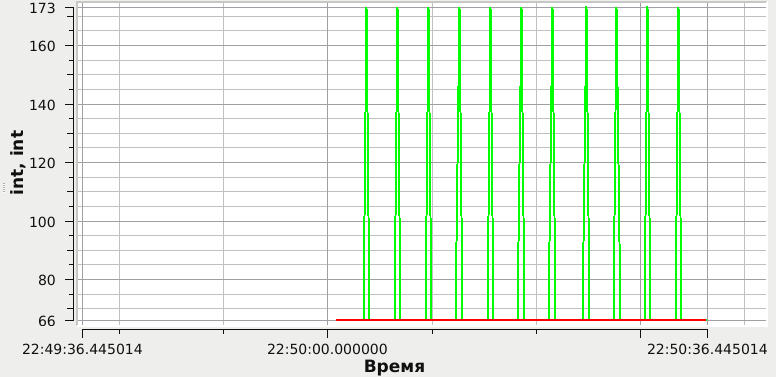
\includegraphics[scale=0.6]{tests/param_bind/graph}
 \caption{График изменения значений параметров (красный - 4а, зелёный - 6а)}
 \label{fig:param_bind_graph}
\end{figure}

\begin{figure}[H]
 \centering
 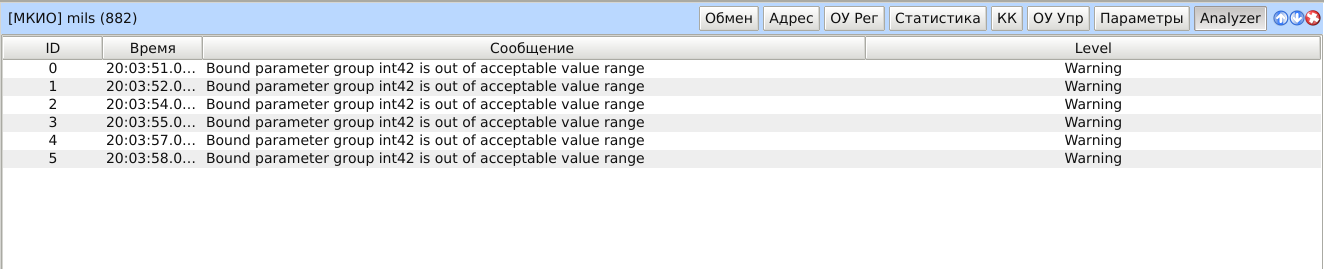
\includegraphics[scale=0.4]{tests/param_bind/report}
 \caption{Результат работы анализатора}
 \label{fig:param_bind_report}
\end{figure}

\subsubsection{Пример 2}

В примере 2 наблюдается изменение значения параметра 6 из 
таблицы~\ref{tab:params}. Для проверки факта равенства параметра ошибочному 
значению 57005 (0xDEAD) используется ограничение error\_value.

График изменения значения параметра 
приводится на рисунке~\ref{fig:param_error_value_graph}. Отчёт анализатора 
приводится на рисунке~\ref{fig:param_error_value_report}.

\lstinputlisting[caption=Пример описания протокола 
2]{tests/param_error_value/protocol.xml}

\begin{figure}[H]
 \centering
 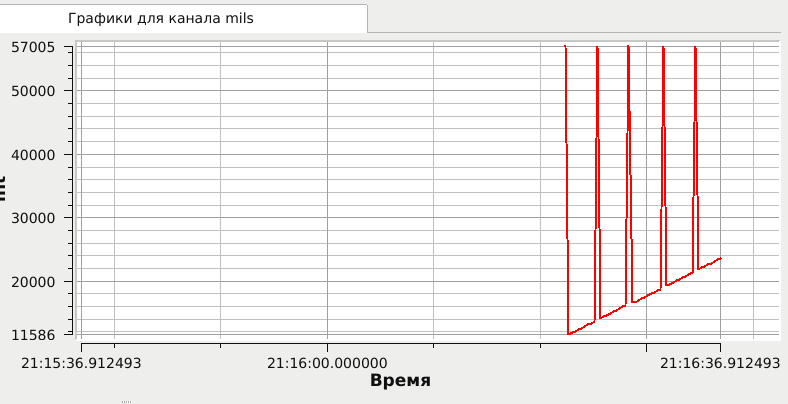
\includegraphics[scale=0.6]{tests/param_error_value/graph}
 \caption{График изменения значений параметра 6}
 \label{fig:param_error_value_graph}
\end{figure}

\begin{figure}[H]
 \centering
 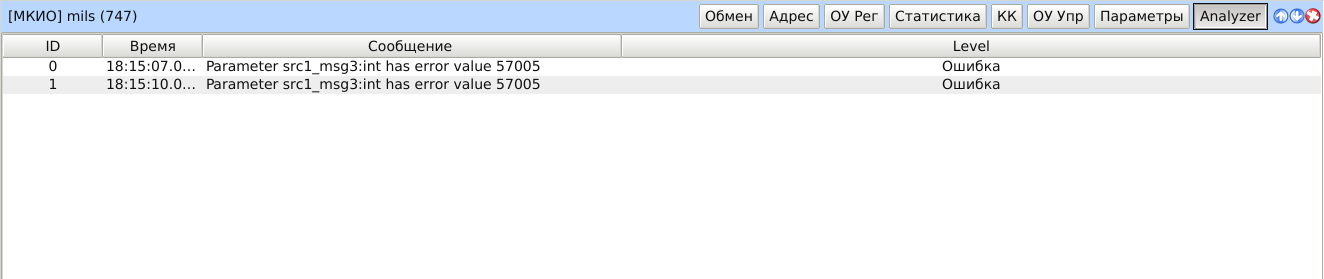
\includegraphics[scale=0.4]{tests/param_error_value/report}
 \caption{Результат работы анализатора}
 \label{fig:param_error_value_report}
\end{figure}

\subsubsection{Пример 3}

В примере 3 наблюдается изменение значения параметра 6 из 
таблицы~\ref{tab:params}. Для обнаружения ``выбросов'' (значительных (>5\%)
отклонений значения параметра от исходной функции) используется ограничение 
smooth с максимальным значением производной по модулю, равным 1000 (значение 
подобрано эмпирически).

График изменения значения параметра 
приводится на рисунке~\ref{fig:param_smooth_graph}. Отчёт анализатора 
приводится на рисунке~\ref{fig:param_smooth_report}.

\lstinputlisting[caption=Пример описания протокола 
3]{tests/param_smooth/protocol.xml}

\begin{figure}[H]
 \centering
 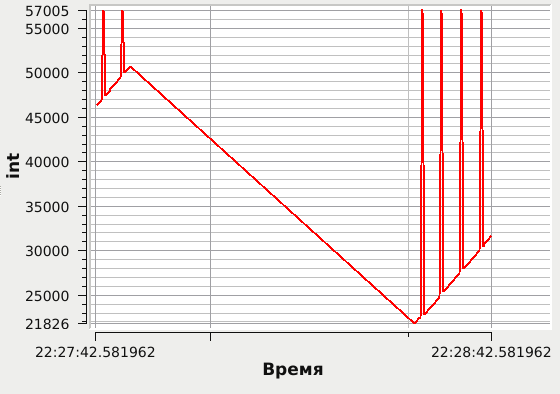
\includegraphics[scale=0.6]{tests/param_smooth/graph}
 \caption{График изменения значений параметра 6}
 \label{fig:param_smooth_graph}
\end{figure}

\begin{figure}[H]
 \centering
 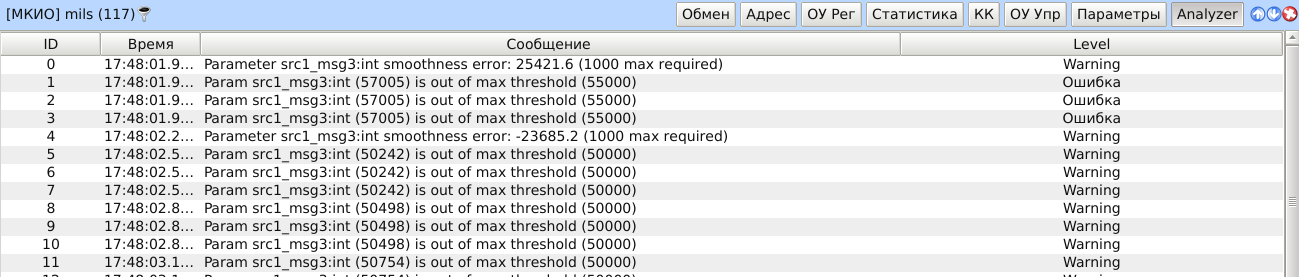
\includegraphics[scale=0.4]{tests/param_smooth/report}
 \caption{Результат работы анализатора}
 \label{fig:param_smooth_report}
\end{figure}

\subsection{Результаты}

В процессе апробации было выяснено, что анализатор корректно обрабатывает 
ограничения, накладываемые на обмены и параметры в описании протокола.

В планах до защиты ВКР есть также апробация анализатора на трассах с 
известными проблемами, зарегистрированных в ходе испытаний на стенде 
[\ref{stand}].